\documentclass[1p]{elsarticle_modified}
%\bibliographystyle{elsarticle-num}

%\usepackage[colorlinks]{hyperref}
%\usepackage{abbrmath_seonhwa} %\Abb, \Ascr, \Acal ,\Abf, \Afrak
\usepackage{amsfonts}
\usepackage{amssymb}
\usepackage{amsmath}
\usepackage{amsthm}
\usepackage{scalefnt}
\usepackage{amsbsy}
\usepackage{kotex}
\usepackage{caption}
\usepackage{subfig}
\usepackage{color}
\usepackage{graphicx}
\usepackage{xcolor} %% white, black, red, green, blue, cyan, magenta, yellow
\usepackage{float}
\usepackage{setspace}
\usepackage{hyperref}

\usepackage{tikz}
\usetikzlibrary{arrows}

\usepackage{multirow}
\usepackage{array} % fixed length table
\usepackage{hhline}

%%%%%%%%%%%%%%%%%%%%%
\makeatletter
\renewcommand*\env@matrix[1][\arraystretch]{%
	\edef\arraystretch{#1}%
	\hskip -\arraycolsep
	\let\@ifnextchar\new@ifnextchar
	\array{*\c@MaxMatrixCols c}}
\makeatother %https://tex.stackexchange.com/questions/14071/how-can-i-increase-the-line-spacing-in-a-matrix
%%%%%%%%%%%%%%%

\usepackage[normalem]{ulem}

\newcommand{\msout}[1]{\ifmmode\text{\sout{\ensuremath{#1}}}\else\sout{#1}\fi}
%SOURCE: \msout is \stkout macro in https://tex.stackexchange.com/questions/20609/strikeout-in-math-mode

\newcommand{\cancel}[1]{
	\ifmmode
	{\color{red}\msout{#1}}
	\else
	{\color{red}\sout{#1}}
	\fi
}

\newcommand{\add}[1]{
	{\color{blue}\uwave{#1}}
}

\newcommand{\replace}[2]{
	\ifmmode
	{\color{red}\msout{#1}}{\color{blue}\uwave{#2}}
	\else
	{\color{red}\sout{#1}}{\color{blue}\uwave{#2}}
	\fi
}

\newcommand{\Sol}{\mathcal{S}} %segment
\newcommand{\D}{D} %diagram
\newcommand{\A}{\mathcal{A}} %arc


%%%%%%%%%%%%%%%%%%%%%%%%%%%%%5 test

\def\sl{\operatorname{\textup{SL}}(2,\Cbb)}
\def\psl{\operatorname{\textup{PSL}}(2,\Cbb)}
\def\quan{\mkern 1mu \triangleright \mkern 1mu}

\theoremstyle{definition}
\newtheorem{thm}{Theorem}[section]
\newtheorem{prop}[thm]{Proposition}
\newtheorem{lem}[thm]{Lemma}
\newtheorem{ques}[thm]{Question}
\newtheorem{cor}[thm]{Corollary}
\newtheorem{defn}[thm]{Definition}
\newtheorem{exam}[thm]{Example}
\newtheorem{rmk}[thm]{Remark}
\newtheorem{alg}[thm]{Algorithm}

\newcommand{\I}{\sqrt{-1}}
\begin{document}

%\begin{frontmatter}
%
%\title{Boundary parabolic representations of knots up to 8 crossings}
%
%%% Group authors per affiliation:
%\author{Yunhi Cho} 
%\address{Department of Mathematics, University of Seoul, Seoul, Korea}
%\ead{yhcho@uos.ac.kr}
%
%
%\author{Seonhwa Kim} %\fnref{s_kim}}
%\address{Center for Geometry and Physics, Institute for Basic Science, Pohang, 37673, Korea}
%\ead{ryeona17@ibs.re.kr}
%
%\author{Hyuk Kim}
%\address{Department of Mathematical Sciences, Seoul National University, Seoul 08826, Korea}
%\ead{hyukkim@snu.ac.kr}
%
%\author{Seokbeom Yoon}
%\address{Department of Mathematical Sciences, Seoul National University, Seoul, 08826,  Korea}
%\ead{sbyoon15@snu.ac.kr}
%
%\begin{abstract}
%We find all boundary parabolic representation of knots up to 8 crossings.
%
%\end{abstract}
%\begin{keyword}
%    \MSC[2010] 57M25 
%\end{keyword}
%
%\end{frontmatter}

%\linenumbers
%\tableofcontents
%
\newcommand\colored[1]{\textcolor{white}{\rule[-0.35ex]{0.8em}{1.4ex}}\kern-0.8em\color{red} #1}%
%\newcommand\colored[1]{\textcolor{white}{ #1}\kern-2.17ex	\textcolor{white}{ #1}\kern-1.81ex	\textcolor{white}{ #1}\kern-2.15ex\color{red}#1	}

{\Large $\underline{12a_{0420}~(K12a_{0420})}$}

\setlength{\tabcolsep}{10pt}
\renewcommand{\arraystretch}{1.6}
\vspace{1cm}\begin{tabular}{m{100pt}>{\centering\arraybackslash}m{274pt}}
\multirow{5}{120pt}{
	\centering
	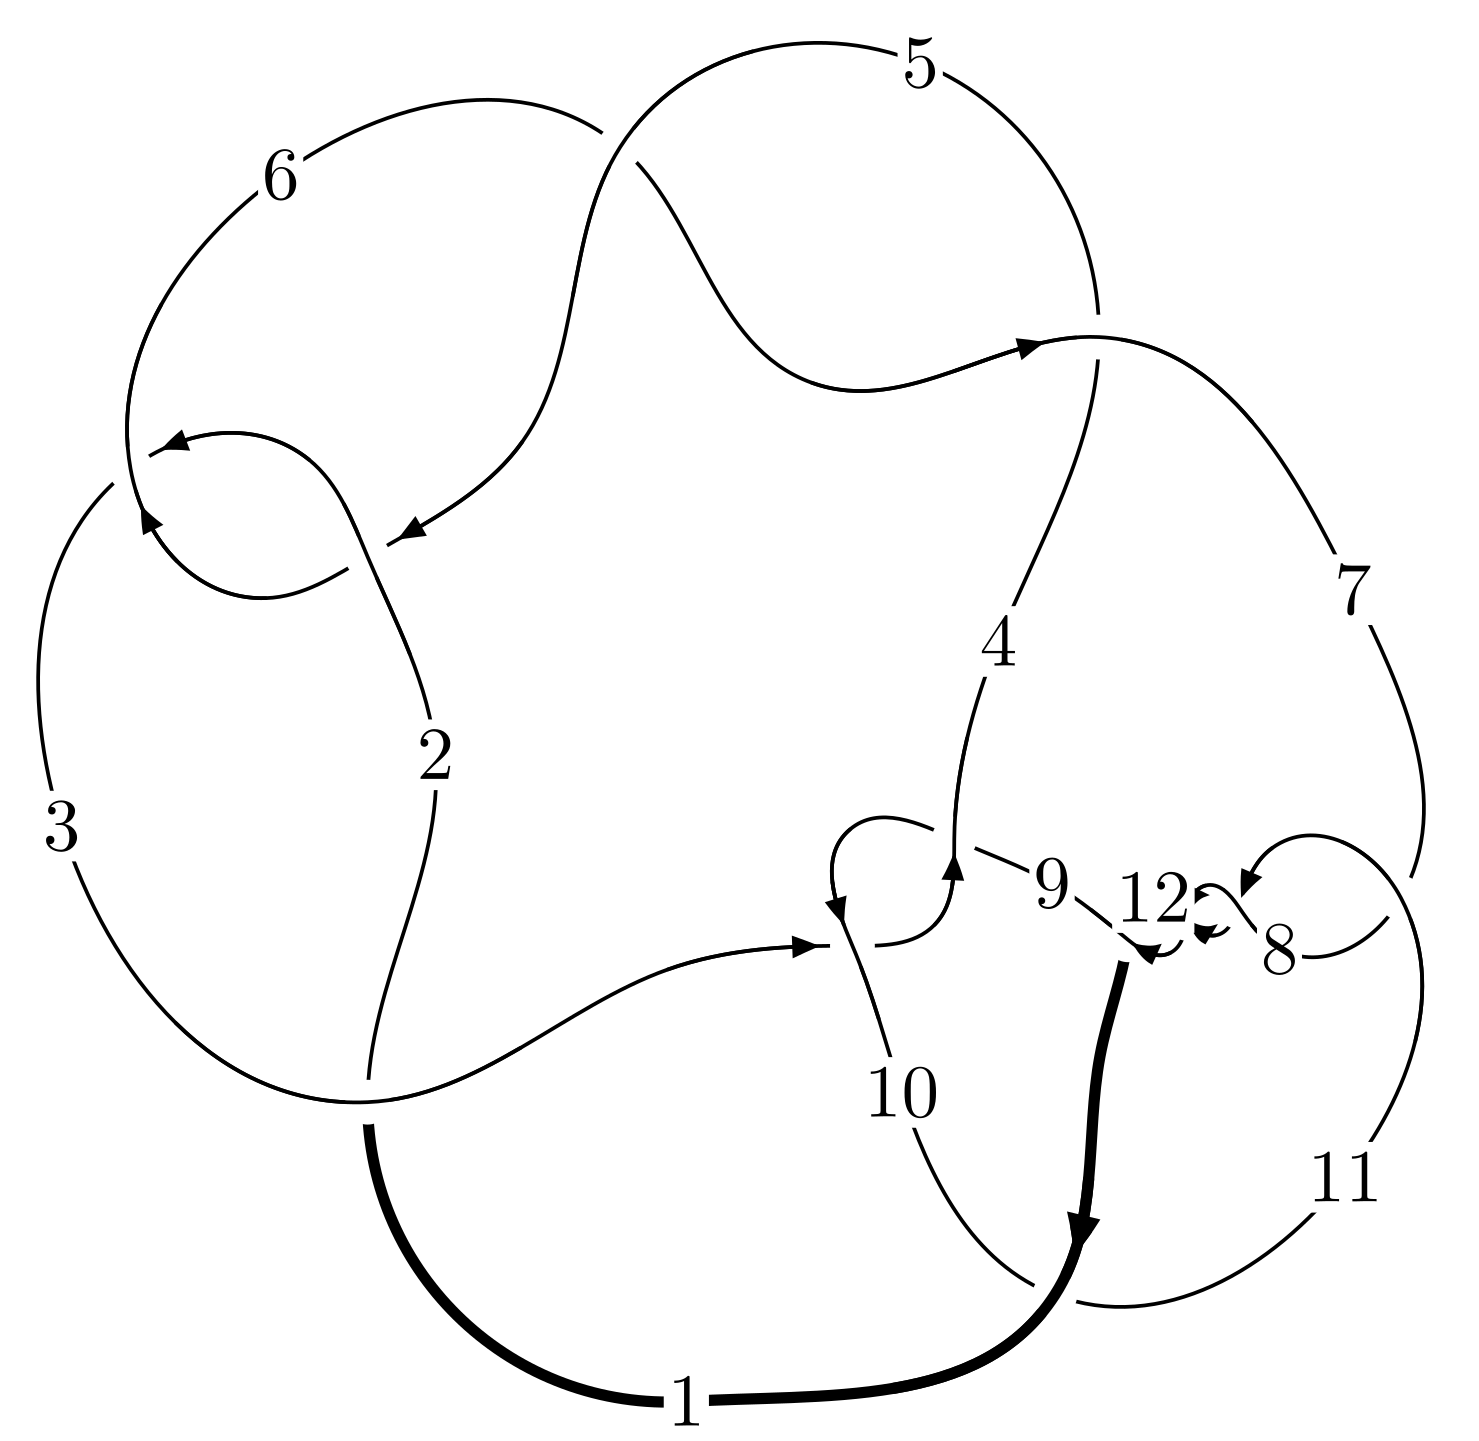
\includegraphics[width=112pt]{../../../GIT/diagram.site/Diagrams/png/1221_12a_0420.png}\\
\ \ \ A knot diagram\footnotemark}&
\allowdisplaybreaks
\textbf{Linearized knot diagam} \\
\cline{2-2}
 &
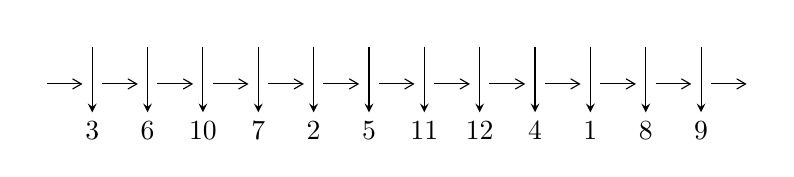
\begin{tikzpicture}[x=20pt, y=17pt]
	% nodes
	\node (C0) at (0, 0) {};
	\node (C1) at (1, 0) {};
	\node (C1U) at (1, +1) {};
	\node (C1D) at (1, -1) {3};

	\node (C2) at (2, 0) {};
	\node (C2U) at (2, +1) {};
	\node (C2D) at (2, -1) {6};

	\node (C3) at (3, 0) {};
	\node (C3U) at (3, +1) {};
	\node (C3D) at (3, -1) {10};

	\node (C4) at (4, 0) {};
	\node (C4U) at (4, +1) {};
	\node (C4D) at (4, -1) {7};

	\node (C5) at (5, 0) {};
	\node (C5U) at (5, +1) {};
	\node (C5D) at (5, -1) {2};

	\node (C6) at (6, 0) {};
	\node (C6U) at (6, +1) {};
	\node (C6D) at (6, -1) {5};

	\node (C7) at (7, 0) {};
	\node (C7U) at (7, +1) {};
	\node (C7D) at (7, -1) {11};

	\node (C8) at (8, 0) {};
	\node (C8U) at (8, +1) {};
	\node (C8D) at (8, -1) {12};

	\node (C9) at (9, 0) {};
	\node (C9U) at (9, +1) {};
	\node (C9D) at (9, -1) {4};

	\node (C10) at (10, 0) {};
	\node (C10U) at (10, +1) {};
	\node (C10D) at (10, -1) {1};

	\node (C11) at (11, 0) {};
	\node (C11U) at (11, +1) {};
	\node (C11D) at (11, -1) {8};

	\node (C12) at (12, 0) {};
	\node (C12U) at (12, +1) {};
	\node (C12D) at (12, -1) {9};
	\node (C13) at (13, 0) {};

	% arrows
	\draw[->,>={angle 60}]
	(C0) edge (C1) (C1) edge (C2) (C2) edge (C3) (C3) edge (C4) (C4) edge (C5) (C5) edge (C6) (C6) edge (C7) (C7) edge (C8) (C8) edge (C9) (C9) edge (C10) (C10) edge (C11) (C11) edge (C12) (C12) edge (C13) ;	\draw[->,>=stealth]
	(C1U) edge (C1D) (C2U) edge (C2D) (C3U) edge (C3D) (C4U) edge (C4D) (C5U) edge (C5D) (C6U) edge (C6D) (C7U) edge (C7D) (C8U) edge (C8D) (C9U) edge (C9D) (C10U) edge (C10D) (C11U) edge (C11D) (C12U) edge (C12D) ;
	\end{tikzpicture} \\
\hhline{~~} \\& 
\textbf{Solving Sequence} \\ \cline{2-2} 
 &
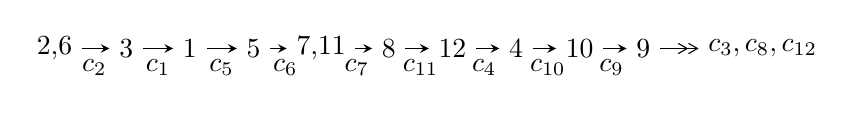
\begin{tikzpicture}[x=23pt, y=7pt]
	% node
	\node (A0) at (-1/8, 0) {2,6};
	\node (A1) at (1, 0) {3};
	\node (A2) at (2, 0) {1};
	\node (A3) at (3, 0) {5};
	\node (A4) at (65/16, 0) {7,11};
	\node (A5) at (41/8, 0) {8};
	\node (A6) at (49/8, 0) {12};
	\node (A7) at (57/8, 0) {4};
	\node (A8) at (65/8, 0) {10};
	\node (A9) at (73/8, 0) {9};
	\node (C1) at (1/2, -1) {$c_{2}$};
	\node (C2) at (3/2, -1) {$c_{1}$};
	\node (C3) at (5/2, -1) {$c_{5}$};
	\node (C4) at (7/2, -1) {$c_{6}$};
	\node (C5) at (37/8, -1) {$c_{7}$};
	\node (C6) at (45/8, -1) {$c_{11}$};
	\node (C7) at (53/8, -1) {$c_{4}$};
	\node (C8) at (61/8, -1) {$c_{10}$};
	\node (C9) at (69/8, -1) {$c_{9}$};
	\node (A10) at (11, 0) {$c_{3},c_{8},c_{12}$};

	% edge
	\draw[->,>=stealth]	
	(A0) edge (A1) (A1) edge (A2) (A2) edge (A3) (A3) edge (A4) (A4) edge (A5) (A5) edge (A6) (A6) edge (A7) (A7) edge (A8) (A8) edge (A9) ;
	\draw[->>,>={angle 60}]	
	(A9) edge (A10);
\end{tikzpicture} \\ 

\end{tabular} \\

\footnotetext{
The image of knot diagram is generated by the software ``\textbf{Draw programme}" developed by Andrew Bartholomew(\url{http://www.layer8.co.uk/maths/draw/index.htm\#Running-draw}), where we modified some parts for our purpose(\url{https://github.com/CATsTAILs/LinksPainter}).
}\phantom \\ \newline 
\centering \textbf{Ideals for irreducible components\footnotemark of $X_{\text{par}}$} 
 
\begin{align*}
I^u_{1}&=\langle 
-2 u^{60}+u^{59}+\cdots+2 b- u,\;2 u^{60}-7 u^{59}+\cdots+2 a+6,\;u^{61}-3 u^{60}+\cdots+6 u-1\rangle \\
I^u_{2}&=\langle 
b- a,\;- u^2 a+a^2- a u- u-1,\;u^3+u^2-1\rangle \\
\\
\end{align*}
\raggedright * 2 irreducible components of $\dim_{\mathbb{C}}=0$, with total 67 representations.\\
\footnotetext{All coefficients of polynomials are rational numbers. But the coefficients are sometimes approximated in decimal forms when there is not enough margin.}
\newpage
\renewcommand{\arraystretch}{1}
\centering \section*{I. $I^u_{1}= \langle -2 u^{60}+u^{59}+\cdots+2 b- u,\;2 u^{60}-7 u^{59}+\cdots+2 a+6,\;u^{61}-3 u^{60}+\cdots+6 u-1 \rangle$}
\flushleft \textbf{(i) Arc colorings}\\
\begin{tabular}{m{7pt} m{180pt} m{7pt} m{180pt} }
\flushright $a_{2}=$&$\begin{pmatrix}1\\0\end{pmatrix}$ \\
\flushright $a_{6}=$&$\begin{pmatrix}0\\u\end{pmatrix}$ \\
\flushright $a_{3}=$&$\begin{pmatrix}1\\u^2\end{pmatrix}$ \\
\flushright $a_{1}=$&$\begin{pmatrix}- u^2+1\\- u^4\end{pmatrix}$ \\
\flushright $a_{5}=$&$\begin{pmatrix}u\\u\end{pmatrix}$ \\
\flushright $a_{7}=$&$\begin{pmatrix}- u^3\\- u^3+u\end{pmatrix}$ \\
\flushright $a_{11}=$&$\begin{pmatrix}- u^{60}+\frac{7}{2} u^{59}+\cdots+\frac{5}{2} u-3\\u^{60}-\frac{1}{2} u^{59}+\cdots+8 u^2+\frac{1}{2} u\end{pmatrix}$ \\
\flushright $a_{8}=$&$\begin{pmatrix}\frac{1}{2} u^{59}- u^{58}+\cdots-\frac{1}{2} u-1\\\frac{1}{2} u^{59}- u^{58}+\cdots+2 u^2+\frac{3}{2} u\end{pmatrix}$ \\
\flushright $a_{12}=$&$\begin{pmatrix}-\frac{1}{2} u^{58}+u^{57}+\cdots-2 u-\frac{3}{2}\\-\frac{1}{2} u^{60}+u^{59}+\cdots+\frac{1}{2} u^2+u\end{pmatrix}$ \\
\flushright $a_{4}=$&$\begin{pmatrix}u^5+u\\u^5- u^3+u\end{pmatrix}$ \\
\flushright $a_{10}=$&$\begin{pmatrix}-2 u^{60}+8 u^{59}+\cdots+12 u-\frac{9}{2}\\\frac{7}{2} u^{60}-3 u^{59}+\cdots+\frac{31}{2} u^2- u\end{pmatrix}$ \\
\flushright $a_{9}=$&$\begin{pmatrix}- u^{59}+\frac{1}{2} u^{58}+\cdots-8 u-\frac{1}{2}\\-\frac{1}{2} u^{60}+\frac{7}{2} u^{58}+\cdots-3 u+1\end{pmatrix}$\\&\end{tabular}
\flushleft \textbf{(ii) Obstruction class $= -1$}\\~\\
\flushleft \textbf{(iii) Cusp Shapes $= -\frac{13}{2} u^{60}+11 u^{59}+\cdots+29 u-\frac{41}{2}$}\\~\\
\newpage\renewcommand{\arraystretch}{1}
\flushleft \textbf{(iv) u-Polynomials at the component}\newline \\
\begin{tabular}{m{50pt}|m{274pt}}
Crossings & \hspace{64pt}u-Polynomials at each crossing \\
\hline $$\begin{aligned}c_{1},c_{4},c_{6}\end{aligned}$$&$\begin{aligned}
&u^{61}+15 u^{60}+\cdots+32 u+1
\end{aligned}$\\
\hline $$\begin{aligned}c_{2},c_{5}\end{aligned}$$&$\begin{aligned}
&u^{61}+3 u^{60}+\cdots+6 u+1
\end{aligned}$\\
\hline $$\begin{aligned}c_{3},c_{9}\end{aligned}$$&$\begin{aligned}
&u^{61}+u^{60}+\cdots+288 u+64
\end{aligned}$\\
\hline $$\begin{aligned}c_{7},c_{8},c_{11}\\c_{12}\end{aligned}$$&$\begin{aligned}
&u^{61}+4 u^{60}+\cdots+u+1
\end{aligned}$\\
\hline $$\begin{aligned}c_{10}\end{aligned}$$&$\begin{aligned}
&u^{61}-14 u^{60}+\cdots+1883 u+233
\end{aligned}$\\
\hline
\end{tabular}\\~\\
\newpage\renewcommand{\arraystretch}{1}
\flushleft \textbf{(v) Riley Polynomials at the component}\newline \\
\begin{tabular}{m{50pt}|m{274pt}}
Crossings & \hspace{64pt}Riley Polynomials at each crossing \\
\hline $$\begin{aligned}c_{1},c_{4},c_{6}\end{aligned}$$&$\begin{aligned}
&y^{61}+65 y^{60}+\cdots+360 y-1
\end{aligned}$\\
\hline $$\begin{aligned}c_{2},c_{5}\end{aligned}$$&$\begin{aligned}
&y^{61}-15 y^{60}+\cdots+32 y-1
\end{aligned}$\\
\hline $$\begin{aligned}c_{3},c_{9}\end{aligned}$$&$\begin{aligned}
&y^{61}+35 y^{60}+\cdots-48128 y-4096
\end{aligned}$\\
\hline $$\begin{aligned}c_{7},c_{8},c_{11}\\c_{12}\end{aligned}$$&$\begin{aligned}
&y^{61}-70 y^{60}+\cdots+33 y-1
\end{aligned}$\\
\hline $$\begin{aligned}c_{10}\end{aligned}$$&$\begin{aligned}
&y^{61}+14 y^{60}+\cdots-820731 y-54289
\end{aligned}$\\
\hline
\end{tabular}\\~\\
\newpage\flushleft \textbf{(vi) Complex Volumes and Cusp Shapes}
$$\begin{array}{c|c|c}  
\text{Solutions to }I^u_{1}& \I (\text{vol} + \sqrt{-1}CS) & \text{Cusp shape}\\
 \hline 
\begin{aligned}
u &= -0.903295 + 0.462746 I \\
a &= -0.695546 - 0.562869 I \\
b &= -0.271804 - 0.008793 I\end{aligned}
 & \phantom{-}1.64912 + 3.33623 I & -8.90726 - 4.06280 I \\ \hline\begin{aligned}
u &= -0.903295 - 0.462746 I \\
a &= -0.695546 + 0.562869 I \\
b &= -0.271804 + 0.008793 I\end{aligned}
 & \phantom{-}1.64912 - 3.33623 I & -8.90726 + 4.06280 I \\ \hline\begin{aligned}
u &= \phantom{-}0.965632 + 0.071466 I \\
a &= \phantom{-}0.255352 - 0.811455 I \\
b &= \phantom{-}0.583357 - 0.467416 I\end{aligned}
 & -1.45506 + 1.38293 I & -14.5746 - 4.7781 I \\ \hline\begin{aligned}
u &= \phantom{-}0.965632 - 0.071466 I \\
a &= \phantom{-}0.255352 + 0.811455 I \\
b &= \phantom{-}0.583357 + 0.467416 I\end{aligned}
 & -1.45506 - 1.38293 I & -14.5746 + 4.7781 I \\ \hline\begin{aligned}
u &= \phantom{-}0.891866 + 0.371875 I \\
a &= \phantom{-}0.025117 + 0.353693 I \\
b &= \phantom{-}0.48374 - 1.47821 I\end{aligned}
 & -9.20574 - 3.82983 I & -18.3699 + 4.7525 I \\ \hline\begin{aligned}
u &= \phantom{-}0.891866 - 0.371875 I \\
a &= \phantom{-}0.025117 - 0.353693 I \\
b &= \phantom{-}0.48374 + 1.47821 I\end{aligned}
 & -9.20574 + 3.82983 I & -18.3699 - 4.7525 I \\ \hline\begin{aligned}
u &= \phantom{-}1.027100 + 0.122511 I \\
a &= -0.577403 + 0.901803 I \\
b &= -1.53356 + 0.54056 I\end{aligned}
 & -8.53214 + 3.20048 I & -17.8758 - 2.0778 I \\ \hline\begin{aligned}
u &= \phantom{-}1.027100 - 0.122511 I \\
a &= -0.577403 - 0.901803 I \\
b &= -1.53356 - 0.54056 I\end{aligned}
 & -8.53214 - 3.20048 I & -17.8758 + 2.0778 I \\ \hline\begin{aligned}
u &= -0.973990 + 0.420575 I \\
a &= \phantom{-}0.605744 + 0.194442 I \\
b &= -0.223113 - 0.672957 I\end{aligned}
 & \phantom{-}0.54572 + 6.96672 I & -12.0000 - 9.8175 I \\ \hline\begin{aligned}
u &= -0.973990 - 0.420575 I \\
a &= \phantom{-}0.605744 - 0.194442 I \\
b &= -0.223113 + 0.672957 I\end{aligned}
 & \phantom{-}0.54572 - 6.96672 I & -12.0000 + 9.8175 I\\
 \hline 
 \end{array}$$\newpage$$\begin{array}{c|c|c}  
\text{Solutions to }I^u_{1}& \I (\text{vol} + \sqrt{-1}CS) & \text{Cusp shape}\\
 \hline 
\begin{aligned}
u &= -1.015250 + 0.392641 I \\
a &= -0.579050 + 0.148607 I \\
b &= \phantom{-}0.52059 + 1.42782 I\end{aligned}
 & -6.92985 + 9.41761 I & -12.0000 - 7.9710 I \\ \hline\begin{aligned}
u &= -1.015250 - 0.392641 I \\
a &= -0.579050 - 0.148607 I \\
b &= \phantom{-}0.52059 - 1.42782 I\end{aligned}
 & -6.92985 - 9.41761 I & -12.0000 + 7.9710 I \\ \hline\begin{aligned}
u &= -0.558526 + 0.717048 I \\
a &= \phantom{-}1.30900 + 0.57411 I \\
b &= \phantom{-}0.615035 + 0.129276 I\end{aligned}
 & -2.84419 + 2.86741 I & -10.16234 - 3.32231 I \\ \hline\begin{aligned}
u &= -0.558526 - 0.717048 I \\
a &= \phantom{-}1.30900 - 0.57411 I \\
b &= \phantom{-}0.615035 - 0.129276 I\end{aligned}
 & -2.84419 - 2.86741 I & -10.16234 + 3.32231 I \\ \hline\begin{aligned}
u &= -0.877865 + 0.718484 I \\
a &= -0.507669 - 0.573262 I \\
b &= -0.710801 - 0.319209 I\end{aligned}
 & \phantom{-}2.45258 + 2.74784 I & \phantom{-0.000000 } 0 \\ \hline\begin{aligned}
u &= -0.877865 - 0.718484 I \\
a &= -0.507669 + 0.573262 I \\
b &= -0.710801 + 0.319209 I\end{aligned}
 & \phantom{-}2.45258 - 2.74784 I & \phantom{-0.000000 } 0 \\ \hline\begin{aligned}
u &= \phantom{-}0.804516 + 0.318031 I \\
a &= \phantom{-}0.196739 - 0.606198 I \\
b &= -0.308799 + 0.790106 I\end{aligned}
 & -1.74945 - 2.32779 I & -16.2262 + 7.6362 I \\ \hline\begin{aligned}
u &= \phantom{-}0.804516 - 0.318031 I \\
a &= \phantom{-}0.196739 + 0.606198 I \\
b &= -0.308799 - 0.790106 I\end{aligned}
 & -1.74945 + 2.32779 I & -16.2262 - 7.6362 I \\ \hline\begin{aligned}
u &= -0.958834 + 0.651543 I \\
a &= \phantom{-}0.741491 + 1.069760 I \\
b &= \phantom{-}1.03234 + 1.20463 I\end{aligned}
 & -3.94098 + 2.19391 I & \phantom{-0.000000 } 0 \\ \hline\begin{aligned}
u &= -0.958834 - 0.651543 I \\
a &= \phantom{-}0.741491 - 1.069760 I \\
b &= \phantom{-}1.03234 - 1.20463 I\end{aligned}
 & -3.94098 - 2.19391 I & \phantom{-0.000000 } 0\\
 \hline 
 \end{array}$$\newpage$$\begin{array}{c|c|c}  
\text{Solutions to }I^u_{1}& \I (\text{vol} + \sqrt{-1}CS) & \text{Cusp shape}\\
 \hline 
\begin{aligned}
u &= -0.808720 + 0.190086 I \\
a &= -1.90972 - 1.06246 I \\
b &= -2.26441 - 0.31552 I\end{aligned}
 & -10.29000 + 0.53665 I & -18.8353 - 9.0691 I \\ \hline\begin{aligned}
u &= -0.808720 - 0.190086 I \\
a &= -1.90972 + 1.06246 I \\
b &= -2.26441 + 0.31552 I\end{aligned}
 & -10.29000 - 0.53665 I & -18.8353 + 9.0691 I \\ \hline\begin{aligned}
u &= -0.761071 + 0.320943 I \\
a &= \phantom{-}1.15383 + 0.94285 I \\
b &= \phantom{-}1.234600 + 0.239084 I\end{aligned}
 & -1.85024 + 1.25608 I & -15.1118 - 4.8976 I \\ \hline\begin{aligned}
u &= -0.761071 - 0.320943 I \\
a &= \phantom{-}1.15383 - 0.94285 I \\
b &= \phantom{-}1.234600 - 0.239084 I\end{aligned}
 & -1.85024 - 1.25608 I & -15.1118 + 4.8976 I \\ \hline\begin{aligned}
u &= \phantom{-}0.898416 + 0.813498 I \\
a &= \phantom{-}1.20213 - 0.99182 I \\
b &= \phantom{-}1.22884 - 0.86819 I\end{aligned}
 & -4.53737 - 3.04417 I & \phantom{-0.000000 } 0 \\ \hline\begin{aligned}
u &= \phantom{-}0.898416 - 0.813498 I \\
a &= \phantom{-}1.20213 + 0.99182 I \\
b &= \phantom{-}1.22884 + 0.86819 I\end{aligned}
 & -4.53737 + 3.04417 I & \phantom{-0.000000 } 0 \\ \hline\begin{aligned}
u &= -0.856068 + 0.862516 I \\
a &= -1.22457 + 2.63205 I \\
b &= \phantom{-}1.20834 + 2.93387 I\end{aligned}
 & -1.50415 - 0.89126 I & \phantom{-0.000000 } 0 \\ \hline\begin{aligned}
u &= -0.856068 - 0.862516 I \\
a &= -1.22457 - 2.63205 I \\
b &= \phantom{-}1.20834 - 2.93387 I\end{aligned}
 & -1.50415 + 0.89126 I & \phantom{-0.000000 } 0 \\ \hline\begin{aligned}
u &= \phantom{-}0.820898 + 0.899902 I \\
a &= -2.06541 - 1.89264 I \\
b &= -0.15813 - 2.95041 I\end{aligned}
 & \phantom{-}1.58971 + 7.54690 I & \phantom{-0.000000 } 0 \\ \hline\begin{aligned}
u &= \phantom{-}0.820898 - 0.899902 I \\
a &= -2.06541 + 1.89264 I \\
b &= -0.15813 + 2.95041 I\end{aligned}
 & \phantom{-}1.58971 - 7.54690 I & \phantom{-0.000000 } 0\\
 \hline 
 \end{array}$$\newpage$$\begin{array}{c|c|c}  
\text{Solutions to }I^u_{1}& \I (\text{vol} + \sqrt{-1}CS) & \text{Cusp shape}\\
 \hline 
\begin{aligned}
u &= -0.886180 + 0.839133 I \\
a &= \phantom{-}1.67113 - 1.82782 I \\
b &= \phantom{-}0.00358 - 2.86721 I\end{aligned}
 & \phantom{-}5.10715 + 1.32327 I & \phantom{-0.000000 } 0 \\ \hline\begin{aligned}
u &= -0.886180 - 0.839133 I \\
a &= \phantom{-}1.67113 + 1.82782 I \\
b &= \phantom{-}0.00358 + 2.86721 I\end{aligned}
 & \phantom{-}5.10715 - 1.32327 I & \phantom{-0.000000 } 0 \\ \hline\begin{aligned}
u &= \phantom{-}0.842192 + 0.896151 I \\
a &= \phantom{-}1.85971 + 1.34927 I \\
b &= \phantom{-}0.56016 + 2.65833 I\end{aligned}
 & \phantom{-}9.11750 + 4.54405 I & \phantom{-0.000000 } 0 \\ \hline\begin{aligned}
u &= \phantom{-}0.842192 - 0.896151 I \\
a &= \phantom{-}1.85971 - 1.34927 I \\
b &= \phantom{-}0.56016 - 2.65833 I\end{aligned}
 & \phantom{-}9.11750 - 4.54405 I & \phantom{-0.000000 } 0 \\ \hline\begin{aligned}
u &= -0.413830 + 0.644735 I \\
a &= -0.606570 - 0.053578 I \\
b &= -0.437841 - 0.476673 I\end{aligned}
 & \phantom{-}3.19857 + 0.74045 I & -5.48051 - 3.33968 I \\ \hline\begin{aligned}
u &= -0.413830 - 0.644735 I \\
a &= -0.606570 + 0.053578 I \\
b &= -0.437841 + 0.476673 I\end{aligned}
 & \phantom{-}3.19857 - 0.74045 I & -5.48051 + 3.33968 I \\ \hline\begin{aligned}
u &= -0.921108 + 0.827807 I \\
a &= -2.24258 + 1.12030 I \\
b &= -1.29799 + 2.86920 I\end{aligned}
 & \phantom{-}4.99860 + 4.88810 I & \phantom{-0.000000 } 0 \\ \hline\begin{aligned}
u &= -0.921108 - 0.827807 I \\
a &= -2.24258 - 1.12030 I \\
b &= -1.29799 - 2.86920 I\end{aligned}
 & \phantom{-}4.99860 - 4.88810 I & \phantom{-0.000000 } 0 \\ \hline\begin{aligned}
u &= \phantom{-}0.864695 + 0.889666 I \\
a &= -1.48550 - 0.77368 I \\
b &= -0.87847 - 2.12723 I\end{aligned}
 & \phantom{-}10.20040 + 0.14626 I & \phantom{-0.000000 } 0 \\ \hline\begin{aligned}
u &= \phantom{-}0.864695 - 0.889666 I \\
a &= -1.48550 + 0.77368 I \\
b &= -0.87847 + 2.12723 I\end{aligned}
 & \phantom{-}10.20040 - 0.14626 I & \phantom{-0.000000 } 0\\
 \hline 
 \end{array}$$\newpage$$\begin{array}{c|c|c}  
\text{Solutions to }I^u_{1}& \I (\text{vol} + \sqrt{-1}CS) & \text{Cusp shape}\\
 \hline 
\begin{aligned}
u &= \phantom{-}0.898542 + 0.870061 I \\
a &= \phantom{-}0.474229 + 0.038157 I \\
b &= \phantom{-}0.796656 + 0.869534 I\end{aligned}
 & \phantom{-}5.34141 - 3.08631 I & \phantom{-0.000000 } 0 \\ \hline\begin{aligned}
u &= \phantom{-}0.898542 - 0.870061 I \\
a &= \phantom{-}0.474229 - 0.038157 I \\
b &= \phantom{-}0.796656 - 0.869534 I\end{aligned}
 & \phantom{-}5.34141 + 3.08631 I & \phantom{-0.000000 } 0 \\ \hline\begin{aligned}
u &= -0.218197 + 0.712691 I \\
a &= \phantom{-}0.502777 + 0.882359 I \\
b &= -0.541108 - 0.948954 I\end{aligned}
 & -4.36643 - 5.46439 I & -10.79014 + 3.37482 I \\ \hline\begin{aligned}
u &= -0.218197 - 0.712691 I \\
a &= \phantom{-}0.502777 - 0.882359 I \\
b &= -0.541108 + 0.948954 I\end{aligned}
 & -4.36643 + 5.46439 I & -10.79014 - 3.37482 I \\ \hline\begin{aligned}
u &= \phantom{-}0.928575 + 0.852722 I \\
a &= -0.522895 - 0.567519 I \\
b &= \phantom{-}0.296827 - 0.457150 I\end{aligned}
 & \phantom{-}5.24177 - 3.29859 I & \phantom{-0.000000 } 0 \\ \hline\begin{aligned}
u &= \phantom{-}0.928575 - 0.852722 I \\
a &= -0.522895 + 0.567519 I \\
b &= \phantom{-}0.296827 + 0.457150 I\end{aligned}
 & \phantom{-}5.24177 + 3.29859 I & \phantom{-0.000000 } 0 \\ \hline\begin{aligned}
u &= -0.952556 + 0.826132 I \\
a &= \phantom{-}2.82339 - 0.54814 I \\
b &= \phantom{-}2.58806 - 2.93805 I\end{aligned}
 & -1.80666 + 7.16585 I & \phantom{-0.000000 } 0 \\ \hline\begin{aligned}
u &= -0.952556 - 0.826132 I \\
a &= \phantom{-}2.82339 + 0.54814 I \\
b &= \phantom{-}2.58806 + 2.93805 I\end{aligned}
 & -1.80666 - 7.16585 I & \phantom{-0.000000 } 0 \\ \hline\begin{aligned}
u &= -0.297713 + 0.668924 I \\
a &= \phantom{-}0.038251 - 0.431492 I \\
b &= \phantom{-}0.427836 + 0.712970 I\end{aligned}
 & \phantom{-}2.69330 - 2.99488 I & -7.10794 + 4.32236 I \\ \hline\begin{aligned}
u &= -0.297713 - 0.668924 I \\
a &= \phantom{-}0.038251 + 0.431492 I \\
b &= \phantom{-}0.427836 - 0.712970 I\end{aligned}
 & \phantom{-}2.69330 + 2.99488 I & -7.10794 - 4.32236 I\\
 \hline 
 \end{array}$$\newpage$$\begin{array}{c|c|c}  
\text{Solutions to }I^u_{1}& \I (\text{vol} + \sqrt{-1}CS) & \text{Cusp shape}\\
 \hline 
\begin{aligned}
u &= \phantom{-}0.963248 + 0.846430 I \\
a &= \phantom{-}1.30769 + 1.41106 I \\
b &= \phantom{-}0.00611 + 2.16662 I\end{aligned}
 & \phantom{-}9.88678 - 6.57001 I & \phantom{-0.000000 } 0 \\ \hline\begin{aligned}
u &= \phantom{-}0.963248 - 0.846430 I \\
a &= \phantom{-}1.30769 - 1.41106 I \\
b &= \phantom{-}0.00611 - 2.16662 I\end{aligned}
 & \phantom{-}9.88678 + 6.57001 I & \phantom{-0.000000 } 0 \\ \hline\begin{aligned}
u &= \phantom{-}0.979698 + 0.836583 I \\
a &= -1.85878 - 1.61789 I \\
b &= -0.64482 - 2.99145 I\end{aligned}
 & \phantom{-}8.68110 - 10.95380 I & \phantom{-0.000000 } 0 \\ \hline\begin{aligned}
u &= \phantom{-}0.979698 - 0.836583 I \\
a &= -1.85878 + 1.61789 I \\
b &= -0.64482 + 2.99145 I\end{aligned}
 & \phantom{-}8.68110 + 10.95380 I & \phantom{-0.000000 } 0 \\ \hline\begin{aligned}
u &= \phantom{-}0.992523 + 0.826283 I \\
a &= \phantom{-}2.32375 + 1.68082 I \\
b &= \phantom{-}1.36651 + 3.55718 I\end{aligned}
 & \phantom{-}1.04634 - 13.93150 I & \phantom{-0.000000 } 0 \\ \hline\begin{aligned}
u &= \phantom{-}0.992523 - 0.826283 I \\
a &= \phantom{-}2.32375 - 1.68082 I \\
b &= \phantom{-}1.36651 - 3.55718 I\end{aligned}
 & \phantom{-}1.04634 + 13.93150 I & \phantom{-0.000000 } 0 \\ \hline\begin{aligned}
u &= \phantom{-}0.584427 + 0.143584 I \\
a &= -0.768708 + 0.414329 I \\
b &= \phantom{-}0.282890 - 0.137929 I\end{aligned}
 & -0.764972 - 0.051966 I & -11.69477 - 1.11358 I \\ \hline\begin{aligned}
u &= \phantom{-}0.584427 - 0.143584 I \\
a &= -0.768708 - 0.414329 I \\
b &= \phantom{-}0.282890 + 0.137929 I\end{aligned}
 & -0.764972 + 0.051966 I & -11.69477 + 1.11358 I \\ \hline\begin{aligned}
u &= \phantom{-}0.327187 + 0.491156 I \\
a &= \phantom{-}1.56928 - 1.31367 I \\
b &= -0.647027 + 0.145084 I\end{aligned}
 & -7.50998 + 0.52039 I & -13.78782 + 1.07094 I \\ \hline\begin{aligned}
u &= \phantom{-}0.327187 - 0.491156 I \\
a &= \phantom{-}1.56928 + 1.31367 I \\
b &= -0.647027 - 0.145084 I\end{aligned}
 & -7.50998 - 0.52039 I & -13.78782 - 1.07094 I\\
 \hline 
 \end{array}$$\newpage$$\begin{array}{c|c|c}  
\text{Solutions to }I^u_{1}& \I (\text{vol} + \sqrt{-1}CS) & \text{Cusp shape}\\
 \hline 
\begin{aligned}
u &= \phantom{-}0.227354\phantom{ +0.000000I} \\
a &= -2.03044\phantom{ +0.000000I} \\
b &= \phantom{-}0.364783\phantom{ +0.000000I}\end{aligned}
 & -0.700986\phantom{ +0.000000I} & -13.7360\phantom{ +0.000000I}\\
 \hline 
 \end{array}$$\newpage\newpage\renewcommand{\arraystretch}{1}
\centering \section*{II. $I^u_{2}= \langle b- a,\;- u^2 a+a^2- a u- u-1,\;u^3+u^2-1 \rangle$}
\flushleft \textbf{(i) Arc colorings}\\
\begin{tabular}{m{7pt} m{180pt} m{7pt} m{180pt} }
\flushright $a_{2}=$&$\begin{pmatrix}1\\0\end{pmatrix}$ \\
\flushright $a_{6}=$&$\begin{pmatrix}0\\u\end{pmatrix}$ \\
\flushright $a_{3}=$&$\begin{pmatrix}1\\u^2\end{pmatrix}$ \\
\flushright $a_{1}=$&$\begin{pmatrix}- u^2+1\\- u^2- u+1\end{pmatrix}$ \\
\flushright $a_{5}=$&$\begin{pmatrix}u\\u\end{pmatrix}$ \\
\flushright $a_{7}=$&$\begin{pmatrix}u^2-1\\u^2+u-1\end{pmatrix}$ \\
\flushright $a_{11}=$&$\begin{pmatrix}a\\a\end{pmatrix}$ \\
\flushright $a_{8}=$&$\begin{pmatrix}- a- u-1\\- a-1\end{pmatrix}$ \\
\flushright $a_{12}=$&$\begin{pmatrix}- u^2 a- a u- u^2- u\\- a u- u^2- u\end{pmatrix}$ \\
\flushright $a_{4}=$&$\begin{pmatrix}1\\u^2\end{pmatrix}$ \\
\flushright $a_{10}=$&$\begin{pmatrix}u^2 a+a u\\a u\end{pmatrix}$ \\
\flushright $a_{9}=$&$\begin{pmatrix}u^2 a+a u\\a u\end{pmatrix}$\\&\end{tabular}
\flushleft \textbf{(ii) Obstruction class $= 1$}\\~\\
\flushleft \textbf{(iii) Cusp Shapes $= u^2 a+2 a u+3 u^2-19$}\\~\\
\newpage\renewcommand{\arraystretch}{1}
\flushleft \textbf{(iv) u-Polynomials at the component}\newline \\
\begin{tabular}{m{50pt}|m{274pt}}
Crossings & \hspace{64pt}u-Polynomials at each crossing \\
\hline $$\begin{aligned}c_{1},c_{4}\end{aligned}$$&$\begin{aligned}
&(u^3- u^2+2 u-1)^2
\end{aligned}$\\
\hline $$\begin{aligned}c_{2}\end{aligned}$$&$\begin{aligned}
&(u^3+u^2-1)^2
\end{aligned}$\\
\hline $$\begin{aligned}c_{3},c_{9}\end{aligned}$$&$\begin{aligned}
&u^6
\end{aligned}$\\
\hline $$\begin{aligned}c_{5}\end{aligned}$$&$\begin{aligned}
&(u^3- u^2+1)^2
\end{aligned}$\\
\hline $$\begin{aligned}c_{6}\end{aligned}$$&$\begin{aligned}
&(u^3+u^2+2 u+1)^2
\end{aligned}$\\
\hline $$\begin{aligned}c_{7},c_{8},c_{10}\end{aligned}$$&$\begin{aligned}
&(u^2+u-1)^3
\end{aligned}$\\
\hline $$\begin{aligned}c_{11},c_{12}\end{aligned}$$&$\begin{aligned}
&(u^2- u-1)^3
\end{aligned}$\\
\hline
\end{tabular}\\~\\
\newpage\renewcommand{\arraystretch}{1}
\flushleft \textbf{(v) Riley Polynomials at the component}\newline \\
\begin{tabular}{m{50pt}|m{274pt}}
Crossings & \hspace{64pt}Riley Polynomials at each crossing \\
\hline $$\begin{aligned}c_{1},c_{4},c_{6}\end{aligned}$$&$\begin{aligned}
&(y^3+3 y^2+2 y-1)^2
\end{aligned}$\\
\hline $$\begin{aligned}c_{2},c_{5}\end{aligned}$$&$\begin{aligned}
&(y^3- y^2+2 y-1)^2
\end{aligned}$\\
\hline $$\begin{aligned}c_{3},c_{9}\end{aligned}$$&$\begin{aligned}
&y^6
\end{aligned}$\\
\hline $$\begin{aligned}c_{7},c_{8},c_{10}\\c_{11},c_{12}\end{aligned}$$&$\begin{aligned}
&(y^2-3 y+1)^3
\end{aligned}$\\
\hline
\end{tabular}\\~\\
\newpage\flushleft \textbf{(vi) Complex Volumes and Cusp Shapes}
$$\begin{array}{c|c|c}  
\text{Solutions to }I^u_{2}& \I (\text{vol} + \sqrt{-1}CS) & \text{Cusp shape}\\
 \hline 
\begin{aligned}
u &= -0.877439 + 0.744862 I \\
a &= -1.071720 - 0.909787 I \\
b &= -1.071720 - 0.909787 I\end{aligned}
 & -5.85852 + 2.82812 I & -16.5384 - 2.7162 I \\ \hline\begin{aligned}
u &= -0.877439 + 0.744862 I \\
a &= \phantom{-}0.409360 + 0.347508 I \\
b &= \phantom{-}0.409360 + 0.347508 I\end{aligned}
 & \phantom{-}2.03717 + 2.82812 I & -19.0485 - 4.3818 I \\ \hline\begin{aligned}
u &= -0.877439 - 0.744862 I \\
a &= -1.071720 + 0.909787 I \\
b &= -1.071720 + 0.909787 I\end{aligned}
 & -5.85852 - 2.82812 I & -16.5384 + 2.7162 I \\ \hline\begin{aligned}
u &= -0.877439 - 0.744862 I \\
a &= \phantom{-}0.409360 - 0.347508 I \\
b &= \phantom{-}0.409360 - 0.347508 I\end{aligned}
 & \phantom{-}2.03717 - 2.82812 I & -19.0485 + 4.3818 I \\ \hline\begin{aligned}
u &= \phantom{-}0.754878\phantom{ +0.000000I} \\
a &= -0.818721\phantom{ +0.000000I} \\
b &= -0.818721\phantom{ +0.000000I}\end{aligned}
 & -2.10041\phantom{ +0.000000I} & -18.9930\phantom{ +0.000000I} \\ \hline\begin{aligned}
u &= \phantom{-}0.754878\phantom{ +0.000000I} \\
a &= \phantom{-}2.14344\phantom{ +0.000000I} \\
b &= \phantom{-}2.14344\phantom{ +0.000000I}\end{aligned}
 & -9.99610\phantom{ +0.000000I} & -12.8330\phantom{ +0.000000I}\\
 \hline 
 \end{array}$$\newpage
\newpage\renewcommand{\arraystretch}{1}
\centering \section*{ III. u-Polynomials}
\begin{tabular}{m{50pt}|m{274pt}}
Crossings & \hspace{64pt}u-Polynomials at each crossing \\
\hline $$\begin{aligned}c_{1},c_{4}\end{aligned}$$&$\begin{aligned}
&((u^3- u^2+2 u-1)^2)(u^{61}+15 u^{60}+\cdots+32 u+1)
\end{aligned}$\\
\hline $$\begin{aligned}c_{2}\end{aligned}$$&$\begin{aligned}
&((u^3+u^2-1)^2)(u^{61}+3 u^{60}+\cdots+6 u+1)
\end{aligned}$\\
\hline $$\begin{aligned}c_{3},c_{9}\end{aligned}$$&$\begin{aligned}
&u^6(u^{61}+u^{60}+\cdots+288 u+64)
\end{aligned}$\\
\hline $$\begin{aligned}c_{5}\end{aligned}$$&$\begin{aligned}
&((u^3- u^2+1)^2)(u^{61}+3 u^{60}+\cdots+6 u+1)
\end{aligned}$\\
\hline $$\begin{aligned}c_{6}\end{aligned}$$&$\begin{aligned}
&((u^3+u^2+2 u+1)^2)(u^{61}+15 u^{60}+\cdots+32 u+1)
\end{aligned}$\\
\hline $$\begin{aligned}c_{7},c_{8}\end{aligned}$$&$\begin{aligned}
&((u^2+u-1)^3)(u^{61}+4 u^{60}+\cdots+u+1)
\end{aligned}$\\
\hline $$\begin{aligned}c_{10}\end{aligned}$$&$\begin{aligned}
&((u^2+u-1)^3)(u^{61}-14 u^{60}+\cdots+1883 u+233)
\end{aligned}$\\
\hline $$\begin{aligned}c_{11},c_{12}\end{aligned}$$&$\begin{aligned}
&((u^2- u-1)^3)(u^{61}+4 u^{60}+\cdots+u+1)
\end{aligned}$\\
\hline
\end{tabular}\newpage\renewcommand{\arraystretch}{1}
\centering \section*{ IV. Riley Polynomials}
\begin{tabular}{m{50pt}|m{274pt}}
Crossings & \hspace{64pt}Riley Polynomials at each crossing \\
\hline $$\begin{aligned}c_{1},c_{4},c_{6}\end{aligned}$$&$\begin{aligned}
&((y^3+3 y^2+2 y-1)^2)(y^{61}+65 y^{60}+\cdots+360 y-1)
\end{aligned}$\\
\hline $$\begin{aligned}c_{2},c_{5}\end{aligned}$$&$\begin{aligned}
&((y^3- y^2+2 y-1)^2)(y^{61}-15 y^{60}+\cdots+32 y-1)
\end{aligned}$\\
\hline $$\begin{aligned}c_{3},c_{9}\end{aligned}$$&$\begin{aligned}
&y^6(y^{61}+35 y^{60}+\cdots-48128 y-4096)
\end{aligned}$\\
\hline $$\begin{aligned}c_{7},c_{8},c_{11}\\c_{12}\end{aligned}$$&$\begin{aligned}
&((y^2-3 y+1)^3)(y^{61}-70 y^{60}+\cdots+33 y-1)
\end{aligned}$\\
\hline $$\begin{aligned}c_{10}\end{aligned}$$&$\begin{aligned}
&((y^2-3 y+1)^3)(y^{61}+14 y^{60}+\cdots-820731 y-54289)
\end{aligned}$\\
\hline
\end{tabular}
\vskip 2pc
\end{document}